\documentclass{article}
\usepackage{tikz}
\usetikzlibrary{calc,patterns,decorations.pathmorphing,decorations.markings}


\begin{document}

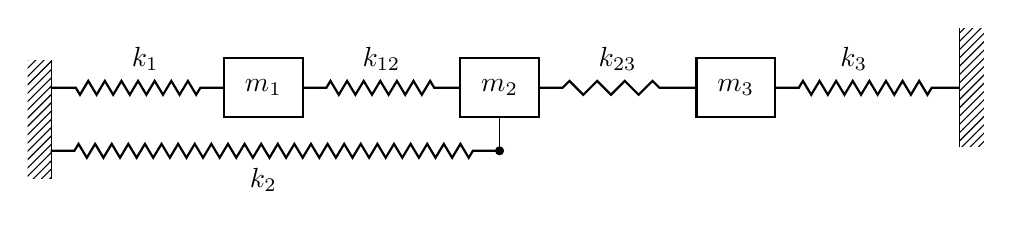
\begin{tikzpicture}[]
\tikzstyle{spring}=[thick,decorate,decoration={zigzag,pre length=0.3cm,post length=0.3cm,segment length=6}]
\tikzstyle{weakspring}=[thick,decorate,decoration={zigzag,pre length=0.3cm,post length=0.3cm,segment length=10}]
\tikzstyle{wall}=[fill,pattern=north east lines,draw=none,minimum width=0.3cm,minimum height=1.5cm]


\node (leftwall)  [wall, xshift=-3cm, yshift=-.4cm,anchor=west] {};
\draw (leftwall.north east) -- (leftwall.south east);

\node(M1)  [minimum width=1cm,minimum height=.75cm, style={draw,outer sep=0pt,thick}] {$m_1$};

\node(M2)  [minimum width=1cm,minimum height=.75cm, xshift = 3 cm,style={draw,outer sep=0pt,thick}] {$m_2$};

\node(M3)  [minimum width=1cm,minimum height=.75cm, xshift =6 cm,style={draw,outer sep=0pt,thick}] {$m_3$};

\node(rightwall)[wall, xshift = 9 cm]{};
\draw (rightwall.north west) -- (rightwall.south west);

\draw [spring] (M1.west)  -- (-3cm+.3cm,0);
\node [above] at (-1.5cm,.1cm) {$k_1$};
\draw[spring](M1.east)--(M2.west);
\node [above] at (1.5cm,.1cm) {$k_{12}$};
\draw[weakspring](M2.east)--(M3.west);
\node [above] at (4.5cm,.1cm) {$k_{23}$};
\draw[spring](M3.east)--(rightwall.west);
\node [above] at (7.5cm,.1cm) {$k_{3}$};

\draw [fill] circle [radius=.05cm, xshift=3cm, yshift=-.8cm] {};  % xshift to match m2

\draw (M2.south)--(3cm,-.8cm);
\draw[spring] (-3cm+.3cm, -.8cm) -- (3cm, -.8cm);
\node[below] at (0,-.9cm) {$k_2$};

%\draw [spring] (leftwall.east) -- (leftwall.east+1cm){k1};

\end{tikzpicture}


\end{document}